\chapter{Rezultate numerice}

\section{Lungimea de \^{i}mpr\u{a}\c{s}tiere pentru c\^{a}teva poten\c{t}iale simple }
Dup\u{a} cum am ar\u{a}tat mai sus, pentru energii joase, coliziunile sunt, \^{i}n esen\c{t}\u{a} \^{i}n regimul de und\u{a} s, adica corespund unei unde \^{i}mpr\u{a}\c{s}tiate izotropic. Mai mult, c\^{a}nd vectorul de und\u{a} relativ $k$ (sau energia $\hbar^2k^2/(2m_r)$) tinde la zero, defazajul $\delta_0(k)$ pentru unda s este propor\c{t}ional cu $k$ (modulo $\pi$) astfel c\u{a} amplitudinea de \^{i}mpr\u{a}\c{s}tiere tinde la o constant\u{a}:
\begin{align}
f(k)\bigg\rvert_{\text{und\u{a} s}}=\frac{e^{i\delta_0k}\sin\delta_0(k)}{k}\to -a \qquad \text{c\^{a}nd} \quad k\to 0 
\end{align}
Solutia problemei de \^{i}mpr\u{a}\c{s}tiere la energii ultra-joase se rezum\u{a} la determinarea unei singure cantit\u{a}\c{t}i: lungimea de \^{i}mpr\u{a}\c{s}tiere $a$.\\

O astfel de determinare se realizeaz\u{a} \^{i}n felul urm\u{a}tor: Scriem ecua\c{t}ia radial\u{a} 
\begin{align}
&\chi''({\bm r})+(\frac{2M}{\hbar^2}(E({\bm k})-U({\bm r}))-\frac{l(l+1}{r^2})\chi({\bm r})=0\label{srad}
\end{align}
pentru $l=0$, pe care o vom integra pe intervalul $r\in (\epsilon,r_{Max})$, unde $\epsilon$ este ales foarte mic, iar $r_{Max}$ este mai mare dec\^at raza de ac\c tiune a potentialului, folosind condi\c tiile la limit\u a
\begin{align}
 &\chi(\epsilon)=\epsilon^{l+1},\quad \chi'(\epsilon)=(l+1)\epsilon^l
\end{align}
Deoarece pentru $r>r_{Max}$ solu\c tia poate fi scris\u a ca o combina\c tie de func\c tii Bessel sferice (Anexa \ref{anexa-bessel}) :
 \begin{align}
&\chi(r_{Max})=A s_l(r_{Max}) +B c_l(r_{Max})\label{eq1}\\
&\chi'(r_{Max})=A s_l'(r_{Max}) +B c_l'(r_{Max})\label{eq2}
\end{align}
unde $s_l(r_{Max})=r_{Max}j_0(k r_{Max})$ \c{s}i $c_l(r_{Max})=r_{Max} y_0 (k r_{Max})$
Putem rezolva sistemul \c{s}i ob\c{t}inem valori pentru constantele $A$ \c{s}i $B$, deci afl\u{a}m $\tan\delta_l=-B/A$. \^{I}n final ob\c{t}inem lungimea de \^{i}mpr\u{a}\c{s}tiere $a$ duc\^{a}ndu-l pe $k$ la zero:
\begin{align}
a=-\lim_{k\to 0}\frac{\tan\delta_0(k)}{k}
\end{align} 
In toate exemplele numerice prezentate \^{i}n continuare vom folosi sistemul de unit\u{a}\c{t}i atomice.

\subsection{Treapta de poten\c{t}ial}

Primul exemplu discutat aici este treapta de poten\c{t}ial, modelat\u{a} de func\c{t}ia:
\begin{align}
V({\bm r})=V(0)\tanh{\frac{{\bm r}-r_0}{\alpha_0}}-V(0)
\end{align}
unde $\alpha_0$ controleaz\u{a} rotunjirea treptei, iar $r_0$ este raza de ac\c{t}iune \c{s}i am ales $M =10^3$ 

Reprezent\u am grafic m\u arimea $-\tan(\delta_0)/k$ ca fun\c tie de $k$ ]c si din grafic putem observa lungimea de \^{\i}mpr\u a\c tiere.
\begin{figure}[h]
\centering
\begin{subfigure}{.5\textwidth}
  \centering
  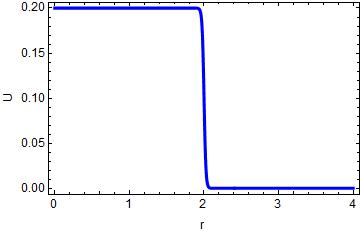
\includegraphics[width=0.9\linewidth]{PotentialTreapta}
  \caption{Poten\c{t}ial Treapt\u{a}}
  \label{fig:sub311}
\end{subfigure}%
\begin{subfigure}{.5\textwidth}
  \centering
  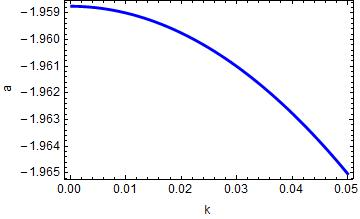
\includegraphics[width=0.9\linewidth]{LungimeImprastiereTreapta}
  \caption{$-\tan(\delta_0)/k$}
  \label{fig:sub312}
\end{subfigure}
\caption{Treapta de poten\c{t}ial}
\label{fig:treapta}
\end{figure}


\subsection{Groapa de poten\c{t}ial}
Al doilea exemplu este groapa de poten\c{t}ial, similar\u{a} cu treapt\u{a}, modelat\u{a} prin aceea\c{s}i func\c{t}ie luat\u{a} cu minus: 
\begin{align}
V({\bm r})=-V(0)\tanh{\frac{{\bm r}-r_0}{\alpha_0}}+V(0)
\end{align}
valorile parametrilor au fost p\u{a}strate
\begin{figure}[h]
\centering
\begin{subfigure}{.5\textwidth}
  \centering
  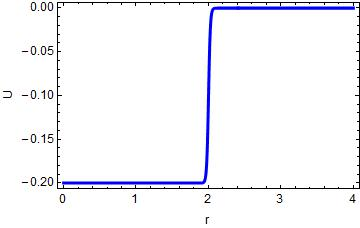
\includegraphics[width=0.9\linewidth]{PotentialGroapa}
  \caption{Poten\c{t}ial Groap\u{a}}
  \label{fig:sub321}
\end{subfigure}%
\begin{subfigure}{.5\textwidth}
  \centering
  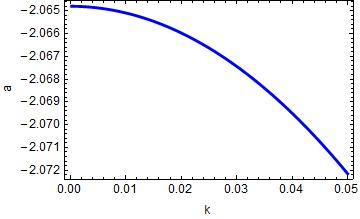
\includegraphics[width=0.9\linewidth]{LungimeImprastiereGroapa}
  \caption{$-\tan(\delta_0)/k$}
  \label{fig:sub322}
\end{subfigure}
\caption{Groapa de poten\c{t}ial}
\label{fig:groapa}
\end{figure}


\subsection{Poten\c{t}ial de tip Van der Waals}
Ultimul exemplu simplu discutat aici este pote\c{t}ialul de tip Van der Waals, modelat de func\c{t}ia:
\begin{align}
U({\bm r})=U(0)\left(\left(\frac{r_0}{{\bm r}}\right)^12-2\left(\frac{r_0}{{\bm r}}\right)^6\right), \qquad \text{unde } U(0)=10^{-6}
\end{align}

\begin{figure}[h]
\centering
\begin{subfigure}{.5\textwidth}
  \centering
  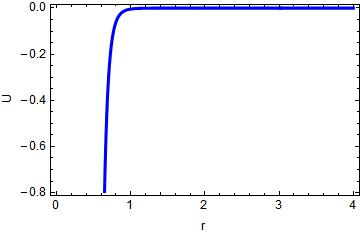
\includegraphics[width=0.9\linewidth]{PotentialVanDerWaals}
  \caption{Poten\c{t}ial de tip Van der Waals}
  \label{fig:sub331}
\end{subfigure}%
\begin{subfigure}{.5\textwidth}
  \centering
  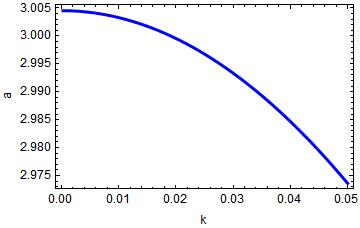
\includegraphics[width=0.9\linewidth]{LungimeImprastiereVanDerWaals}
  \caption{$-\tan(\delta_0)/k$}
  \label{fig:sub332}
\end{subfigure}
\caption{Poten\c{t}ial de tip Van der Waals}
\label{fig:groapa}
\end{figure}


\section{Poten\c{t}ial aproximat pentru atomi de Cs}

Pentru a realiza calculul numeric al defazajelor \^{i}n und\u{a} s \c{s}i a lungimilor de \^{i}mpr\u{a}\c{s}tiere adopt\u{a}m urm\u{a}toarea expresie a poten\c{t}ialului pentru interac\c{t}ia atomilor de Cs:
\begin{align}
U(r)=\frac{1}{2}Br^\alpha e^{-\beta r}-\left(\frac{C_6}{r^6}+\frac{C_8}{r^8}+\frac{C_{10}}{r^{10}}\right)f_c(r)\label{vcs}
\end{align}
Primul termen de dup\u{a} egal reprezint\u{a} repulsia dintre electronii de valen\c{t}\u{a}, iar al doilea reprezint\u{a} suma termenilor Van der Waals, \^{i}nmul\c{t}it\u{a} cu o func\c{t}ie de cutoff $f_c(r)$, ce are rolul de a anula divergen\c{t}a $1/r^n$ la distan\c{t}e mici.\\
Func\c{t}ia de cutoff are forma:
\begin{align}
f_c(r)=\Theta(r-r_c)+\Theta(r_c-r)e^{-(rc/r-1)^2},
\end{align}
unde $\Theta(x)$ reprezint\u{a} func\c{t}ia Heaviside ($\Theta(x)=1,\quad x>0$ \c{s}i $\Theta(x)=0,\quad x<0$)
Parametrii poten\c{t}ialului au fost ale\c{s} din literatur\u{a} \cite{art-VW} (date \^{i}n unit\u{a}\c{t}i atomice):
\begin{center}
 \begin{tabular}{||c c c c c c c||} 
 \hline
 B & $\alpha$ & $\beta$ & $C_6$ & $C_8$ & $C_{10}$ & $r_c$ \\ [0.5ex] 
 \hline 
 0.0016 & 5.53 & 1.072 & 7020 & $1.1 \times 10^6$ & $1.7 \times 10^8$ & 23.165 \\ 
  \hline
\end{tabular}
\end{center}

Situa\c tia este diferit\u a  \^{\i}n acest  caz; un grafic al poten\c tialului
\begin{figure}[h]
  \centering
  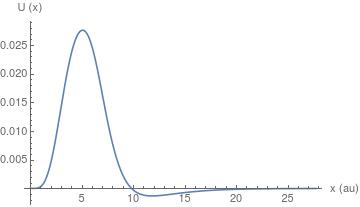
\includegraphics[scale = 0.8]{CS.jpg}
  {\caption{Potentialul (\ref{vcs})\label{gvcs}}}
  \end{figure}
  face u]c sor de \^{\i}n\c teles c\u a prezen\c ta barierei inatl\u a \c si larg\u a faca ca la energii mici propagarea solu\c tiei ``pe sub barier\u a'' sa duc\u a la pierderea complet\u a a preciziei.
  De exemplu \^{\i}n figura \ref{figpsi} este reprezentat\u a solu\c tia $\chi(r)$ g\u asit\u a cu Mathematica pentru $k=0.05$ u.a. E evident c\u a solu\c tia nu are comportarea corect\u a la distan\c te mari.
\begin{figure}[h]
  \centering
  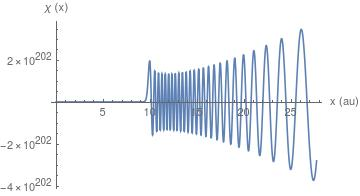
\includegraphics[scale = 0.8]{FIG.jpg}
  {\caption{Potentialul (\ref{vcs})\label{figpsi}}}
  \end{figure}

  
In acest caz sunt mai potrivite metode de evaluare a defazajului bazate pe aproxima\c tia JWKB sau pe calculul direct al fazei solu\c tiei radiale, cum ar fi \cite{ris}, care furnizeaz\u a rezultate in acord cu cele din \cite{art-VW}. 



 

%%% Local Variables:
%%% mode: latex
%%% TeX-master: "../RE"
%%% End:
